\subsection{Термины и определения}

Русскоязычная терминология в области параллельных вычислений (ПВ) не всегда однозначно соответствует англоязычной, поэтому ниже для каждого термина даётся его англоязычный вариант и делается поправка на неидентичность этих терминов, где это необходимо.  

\textbf{Параллельные вычисления (concurrent computing)} -- способ организации вычислений на одном или нескольких компьютерах, при котором пересекаются периоды жизни нескольких задач. Антонимом этого термина являются {\bfseries последовательные вычисления (sequential computing)}, при выполнении которых периоды жизни задач не пересекаются. Например, пусть $start_i$, $end_i$ - это соответственно времена начала и конца жизни вычислительной задачи $i$, и пусть ${start_1 < start_2}$, тогда:

\begin{itemize}
    \item при $end_1 < start_2$ имеют место последовательные вычисления;
    \item при $end_1 \ge start_2$ имеют место параллельные вычисления.
\end{itemize}

Англоязычный термин \textbf{parallel computing} переводится на русский язык тем же словосочетанием: параллельные вычисления. Однако в него вкладывается более узкий, чем в concurrent computing, смысл: при parallel computing задачи исполняются физически одновременно на различных процессорах и/или ядрах одного компьютера. Это значит, что понятие concurrent включает в себя parallel, а именно: любые parallel-вычисления являются concurrent, но не всякие concurrent-вычисления являются parallel.

Классический пример concurrent-вычислений, которые не являются parallel, -- это реализация многозадачности в операционной системе (ОС) при наличии только одного одноядерного процессора. В этом случае ОС не может физически параллельно выполнять разные задачи и вынуждена запускать их в режиме разделения времени, т.е. поочерёдно разрешая использовать процессор разным задачам, переключаясь с задачи на задачу по несколько раз до окончания выполнения каждой из них.

Иногда parallel computing переводится как \textbf{многоядерные вычисления (multicore computing)}, чтобы подчеркнуть отличие от con\-current computing, однако этот термин неидеален, т.к. не позволяет корректно классифицировать вычисления на многопроцессорных компьютерах, в которых каждый процессор является одноядерным. Такие компьютеры позволяют выполнять parallel computing, но не multicore computing. Но этой проблемой можно пренебречь, т.к. подобных компьютеров в данный момент практически нет на рынке. Более точным термином можно считать SMP (shared memory processing), который относится к работе параллельных программ на системах с общей памятью. В таких системах все процессоры/ядра совместно используют общую оперативную память одного компьютера. Итак, можно установить следующие пары соответствий:

\begin{itemize}
    \item параллельные вычисления $\neq$ parallel computing;			
    \item параллельные вычисления $=$ concurrent computing;
    \item многоядерные вычисления $=$ parallel computing;
    \item parallel computing $=$ multicore computing $=$ SMP.
\end{itemize}

\textbf{Распределённые вычисления (distributed computing)} -- такие ПВ, при которых для решения задачи вычисления происходят на процессорах, расположенных на разных компьютерах, соединённых сетью, т.е. для выполнения вычислений приходится передавать программы и/или данные по сети.

Классификация ПВ по особенностям аппаратной реализации:

\begin{enumerate}
    \sloppy
    \item\textbf{Параллелизм на уровне битов} -- процессор выполняет операцию для всех битов машинного слова одновременно. Например, 64-разрядный процессор может одновременно инвертировать значение каждого из 64 битов заданного операнда.
    \item\textbf{Параллелизм на уровне операндов} -- одна инструкция процессора позволяет выполнить некоторую операцию для целого массива операндов параллельно. Например, с помощью технологии SSE за одну операцию можно попарно перемножить элементы двух массивов. (все умножения будут выполнены параллельно во времени). 
    \item\textbf{Параллелизм на уровне инструкций} -- выполнение каждой инструкции разбивается на фазы, каждая из которых может выполняться процессором физически параллельно. Это изменение архитектуры процессора никак не влияет на общее время выполнения одной изолированной инструкции, однако при обработке нескольких подряд идущих инструкций удаётся организовать из них конвейер. В результате подряд идущие инструкции выполняются физически параллельно, что позволяет увеличить общую производительность процессора, выраженную в инструкциях/с (см. детали ниже в этом разделе).
\end{enumerate}

%\par\sout{Важно различать понятия ''параллельные вычисления'' и ''параллельные технологии''. Разберем следующие понятия, которые, хотя и являются параллельными технологиями (на уровне ядра или межъядерного взаимодействия), однако не являются параллельными вычислениями, но часто \textbf{по ошибке} причисляются к ним}:

Перечисленные далее параллельные технологии в данном пособии рассматриваются кратко, чуть шире, чем определения.

\begin{itemize}
    \sloppy
    \item\textit{Конвейерная обработка данных (суперскалярность)} представляет собой одновременную обработку процессором нескольких инструкций, при котором в один момент времени для каждой из инструкций выполняется различный этап выполнения. Например, если какой-либо процессор может одновременно получать, раскодировать и выполнить инструкцию, то он во время получения первой инструкции может раскодировать вторую и выполнять третью (рисунок~\ref{pipelineExample:image}). Этот способ организации вычислений не является параллельными вычислениями, потому что инструкции все равно выполняются последовательно, а задействовано только одно ядро.
    
    \begin{figure}[H]
         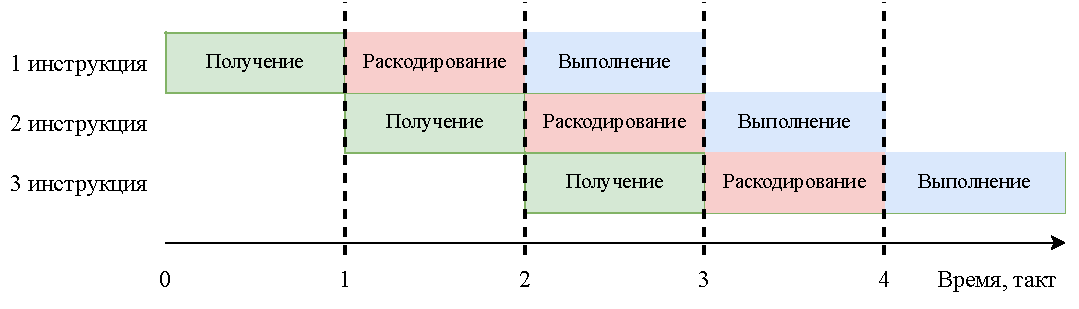
\includegraphics[width=\linewidth]{simd-pipeline}
         \caption{\textit{Конвейерная обработка инструкций}}
         \label{pipelineExample:image}
    \end{figure}
    
    \item\textit{SIMD-расширения (MMX, SSE)} обеспечивают параллелизм на уровне данных. Например, процессор может одновременно умножать четыре числа вместо одного с помощью SSE инструкции. Однако поток команд все равно остается одиночным, т.е. выполняется одна инструкция программы за промежуток времени, что не является случаем параллельных вычислений.
    \item\textit{Вытесняющая многозадачность} организуется операционной системой. Несколько процессов стоят в очереди выполнения и ОС сама решает как распорядиться процессорным временем между ними. Если у первого потока задан больший приоритет, чем у второго, то ОС будет выделять больше времени на выполнение первого потока, однако в один момент времени будет выполняться только один поток, следовательно, вытесняющая многозадачность тоже не входит в понятие параллельных вычислений.
\end{itemize}

Для организации параллельных вычислений используются различные технологии распараллеливания:

\begin{itemize}
    \item\textbf{Process (процесс)} -- наиболее тяжеловесный механизм, применяемый для распараллеливания. Каждый процесс имеет свое независимое адресное пространство, поэтому синхронизация данных между процессами долгая и сложная. Может включать в себя несколько потоков исполнения.
    \item\textbf{Thread (поток исполнения, нить, тред, поток)} выполняется независимо от других потоков, но имеет общее адресное пространство с другими потоками в рамках одного процесса. На этом уровне используется механизмы синхронизации данных (будут рассмотрены далее).
    \item\textbf{Fiber (волокно)} -- легковесный поток выполнения. Также как и треды, fiber'ы имеют общее адресное пространство, однако используют совместную многозадачность вместо вытесняющей. ОС не переключает контекст из одного треда в другой, вместо этого главный поток сам выделяет время для работы дочернего fiber, либо блокируется логически (то есть жизненным циклом fiber'a управляет программист). Также все fiber'ы работают на одном ядре, в отличие от тредов, которые могут работать на разных ядрах.
\end{itemize}

Для лучшего понимания тредов схематично рассмотрим его жизненный цикл (lifecycle). На рисунке~\ref{threadLifecycle:image} видно, что поток может находиться в трех состояниях -- готовность, ожидание и выполнение. После создания потока он пребывает в состоянии готовности. Затем ОС принимает решение о смене его состояния (вытесняющая многозадачность). Для fiber жизненный цикл такой же, но переходами между ними управляет программист или механизмы синхронизации.

Разные стандарты языков программирования могут добавлять в жизненный цикл потоков новые состояния, например, блокировка потока, прерывание работы потока и остальные, однако общая схема работы остается той же.

\begin{figure}[H]
    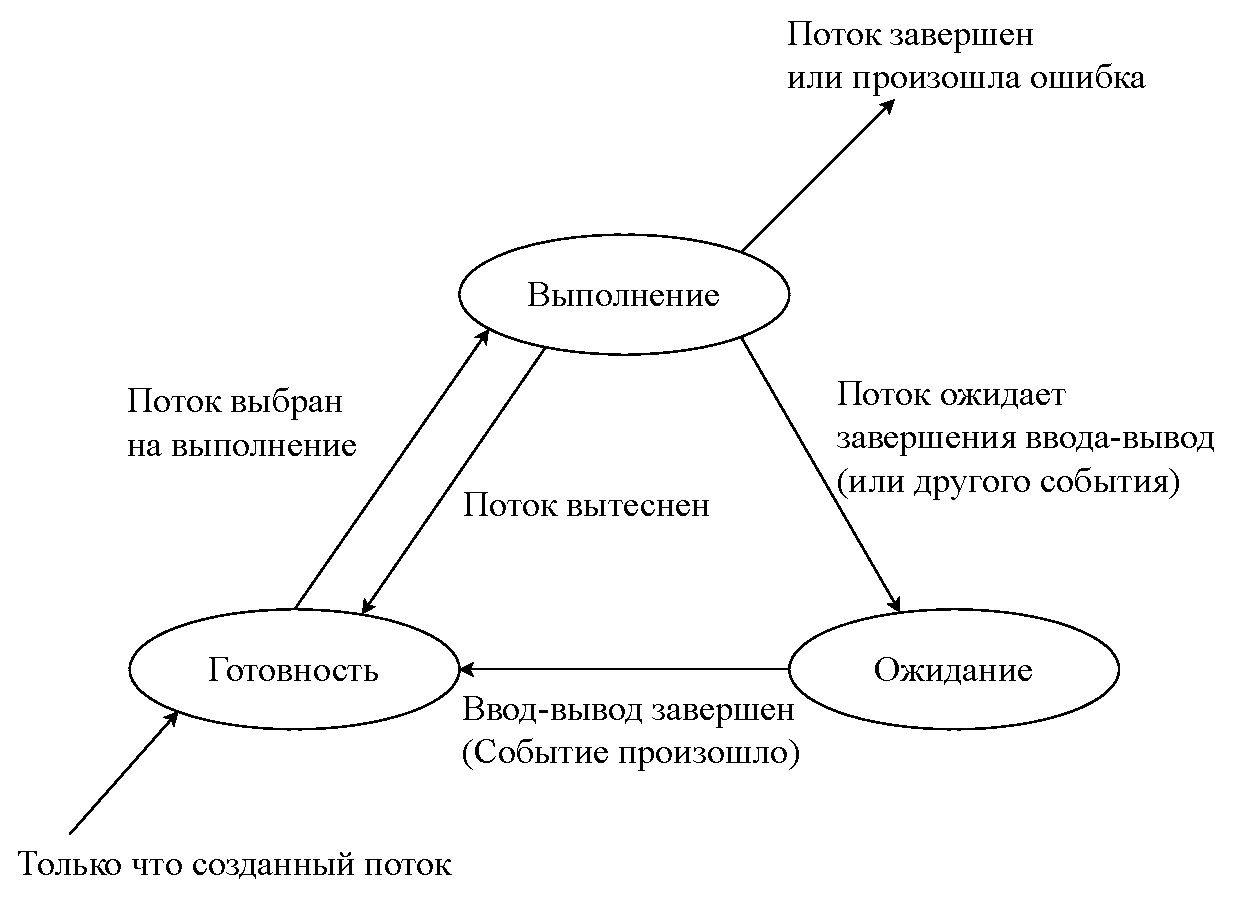
\includegraphics[width=\linewidth]{thread_lifecycle}
    \caption{Жизненный цикл потока}
    \label{threadLifecycle:image}
\end{figure}

\sloppy
В среде программистов существуют понятия \textbf{потокобезопасной (thread-safe)} и \textbf{реентерабельной (reentrant или reenterable)} функции, однако в разных сообществах они могут иметь различные значения. В таблице~\ref{threadSafeReentrant:table} написаны определения из разных источников.

\begin{table}[H]
    \caption{Определения thread-safe и reentrant функций}
    \label{threadSafeReentrant:table}
    \begin{tabularx}{\textwidth}{|c|C|C|}
        \hline
        \thead{Источник \\ определения} & \thead{Thread-safe} & \thead{Reentrant} \\ \hline
        QT & Внутри функции обращение ко всем общим переменным осуществляется строго последовательно, а не параллельно (Thread-safe является reentrant, но не наоборот) & При вызове функции одновременно несколькими потоками гарантируется правильная работа, только если потоки не используют общие данные \\ \hline
        Linux & Функция показывает правильные результаты, даже если вызвана несколькими тредами одновременно & Функция показывает правильные результаты, даже если повторно вызвана изнутри себя \\ \hline
        POSIX &  & Функция показывает правильные результаты, даже если вызвана несколькими тредами одновременно \\ \hline
    \end{tabularx}
\end{table}

Рассмотрим примеры функций, подходящие под определение сообщества Linux.
\inputminted{c++}{listings/swapExample1.cpp}

Данная функция не является ни потокобезопасной, ни реентерабельной, потому что все потоки, вызывающие ее, будут использовать общую переменную t. Если вызвать функцию внутри ее самой, то перезапишется значение t и родительская функция отработает неправильно. Попробуем исправить эти ошибки, объявив переменную t типа \_\_thread int.

\inputminted{c++}{listings/swapExample2.cpp}

Теперь компилятор создаст копию переменной для каждого потока t, и функция станет потокобезопасной, однако она все еще не реентерабельной по той же причине. Будем сохранять значение глобальной переменной t в начале функции и восстанавливать ее в конце.

\inputminted{c++}{listings/swapExample3.cpp}

Новая функция реентерабельна, но снова потоконебезопасна. Наконец, приведем пример реализации swap(), которая потокобезопасна и реентерабельна:

\inputminted{c++}{listings/swapExample4.cpp}
